\documentclass[a4paper]{article}

\usepackage[english]{babel}
\usepackage[utf8]{inputenc}
\usepackage{amsmath}
\usepackage{amssymb}
\usepackage{graphicx}
\usepackage[colorinlistoftodos]{todonotes}
\usepackage[a4paper, total={6in, 9in}]{geometry}
\usepackage{hyperref}
\usepackage{subcaption}
\captionsetup{compatibility=false}

\title{\textbf{Vizualizacija Julijevog skupa} \\ 
      {\large Laboratorijska vježba iz računalne grafike}}

\author{Antun Magdić}

\date{22. siječnja 2021.}

\begin{document}
\maketitle

\section{Teorijska pozadina}

Matematički korektna definicija Julijevog skupa može se pronaći u 
\cite{juliaset}. U ovoj laboratorijskoj vježbi korišteni su Julijevi skupovi
dobiveni iteracijom kvadratnih kompleksnih polinoma. Radi se o funkcijama 
$f: \mathbb{C} \rightarrow \mathbb{C}$ oblika
$$f(z) = z^2 + c,$$
gdje je $c$ neki kompleksan broj. Definiramo pravilo za generiranje niza $(z_n)$
sljedećim izrazom 
$$z_n = f(z_{n-1}) = z_{n-1}^2 + c.$$
Ovisno o prvom elementu niza $z_0$ ovaj niz može biti ograničen i u tom slučaju 
može konvergirati ili ne mora. Ako niz nije ograničen onda divergira. Definiramo
skup $S(c)$ kao skup svih kompleksnih brojeva $z_0$ za koje niz $(z_n)$ 
divergira. Julijev skup $J(c)$ tada je granica skupa $S(c)$. Julijev skup može 
biti povezan ili potpuno nepovezan, a to ovisi o divergenciji niza za $z_0 = 0$. 
Odavde dolazi veza Julijevog i Mandelbrotovog skupa \cite{mandelbrotset}, 
odnosno Julijev skup $J(c)$ je povezan, ako i samo ako $c$ pripada 
Mandelbrotovom skupu.

Julijev skup jedan je od ključnih pojmova u teoriji dinamičkih sustava koji 
često pokazuju kaotično ponašanje. Osim u zbog svoje primjene u matematici 
Julijev skup postao je poznat i po svojoj estetskoj ljepoti i fraktalnoj 
strukturi.

\section{Opis razvijenog programa}

Razvijeni program crta i animira Julijev skup. Program se pokreće iz naredbenog 
retka sa dva argumenta: udaljenosti $r$ kompleksnog broja $c$ od ishodišta i 
opcijom \texttt{bw} ili \texttt{colorful}. Nakon pokretanja animacije počinje.
Za početnu vrijednost parametra $c$ uzima se $r$. Kako prolazi vrijeme $c$ kruži
oko ishodišta nekom frekvencijom $\omega$, odnosno nakon što je prošlo $t$ 
vremena od pokretanja animacije, vrijednost broja $c$ je $r e^{i \omega t}$. Na 
taj način $c$ se stalno nalazi na udaljenosti $r$ od ishodišta. Izgled Julijevog
skupa se mijenja kako $c$ kruži oko ishodišta i ovisno o tome pripada li $c$
Mandelbrotovom skupu, Julijev skup je povezan ili nepovezan.

Za vrijeme rada programa, tipkama na tipkovnici moguće je upravljati slikom na 
ekranu. Dostupne su sljedeće mogućnosti:
\begin{itemize}
    \item \texttt{<RAZMAKNICA>} pokreće i pauzira animaciju,
    \item \texttt{<STRELICA UDESNO>} premotava animaciju unaprijed,
    \item \texttt{<STRELICA ULIJEVO>} premotava animaciju unatrag,
    \item \texttt{d} pomiče kameru u smjeru $1$,
    \item \texttt{w} pomiče kameru u smjeru $+i$,
    \item \texttt{a} pomiče kameru u smjeru $-1$,
    \item \texttt{s} pomiče kameru u smjeru $-i$,
    \item \texttt{i} povećava sliku,
    \item \texttt{o} smanjuje sliku,
    \item \texttt{p} ispisuje trenutnu vrijednost $c$.
\end{itemize}

Na slici \ref{fig:program_example} prikazani su neki primjeri Julijevih skupova.

\begin{figure}
    \centering
    \begin{subfigure}[b]{0.45\textwidth}
        \centering
        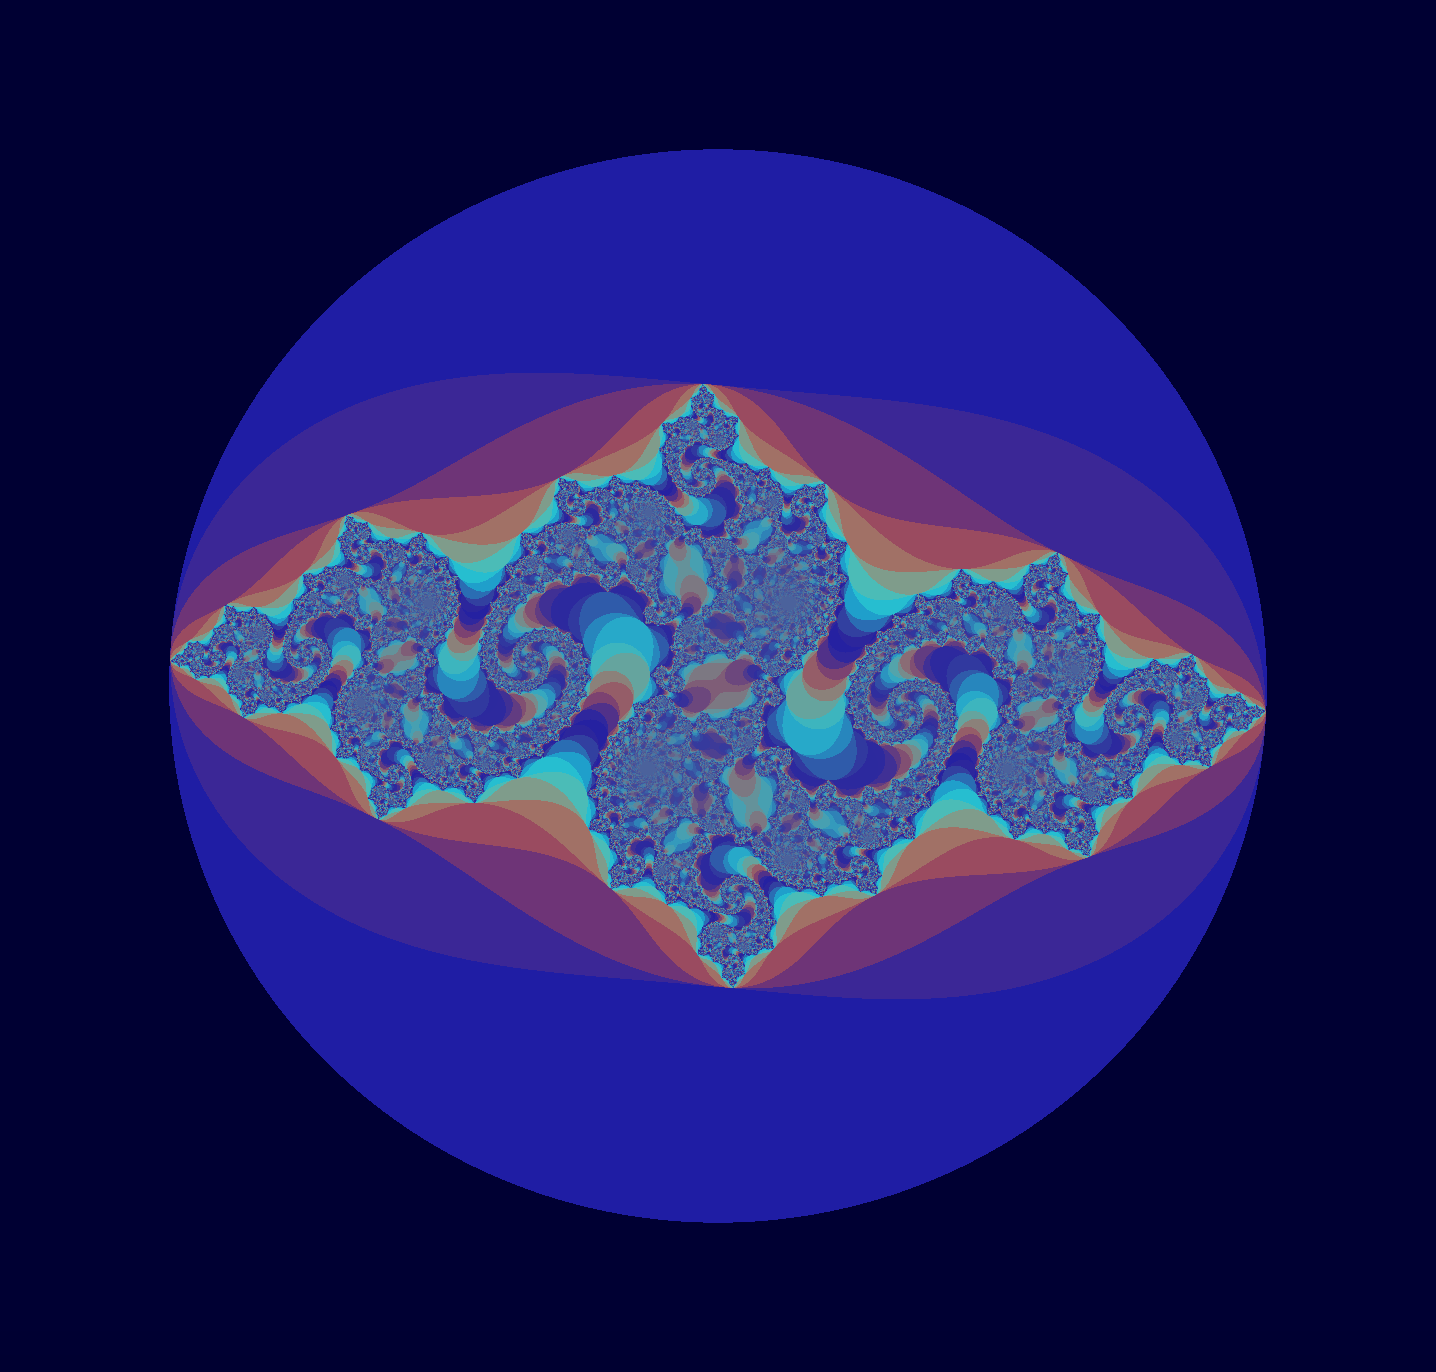
\includegraphics[width=\textwidth]{images/colorful1.png}
    \end{subfigure}
    \hfill
    \begin{subfigure}[b]{0.45\textwidth}
        \centering
        
\includegraphics[width=\textwidth]{images/colorful2.png}
    \end{subfigure}
    \vskip\baselineskip
    \begin{subfigure}[b]{0.45\textwidth}
        \centering
        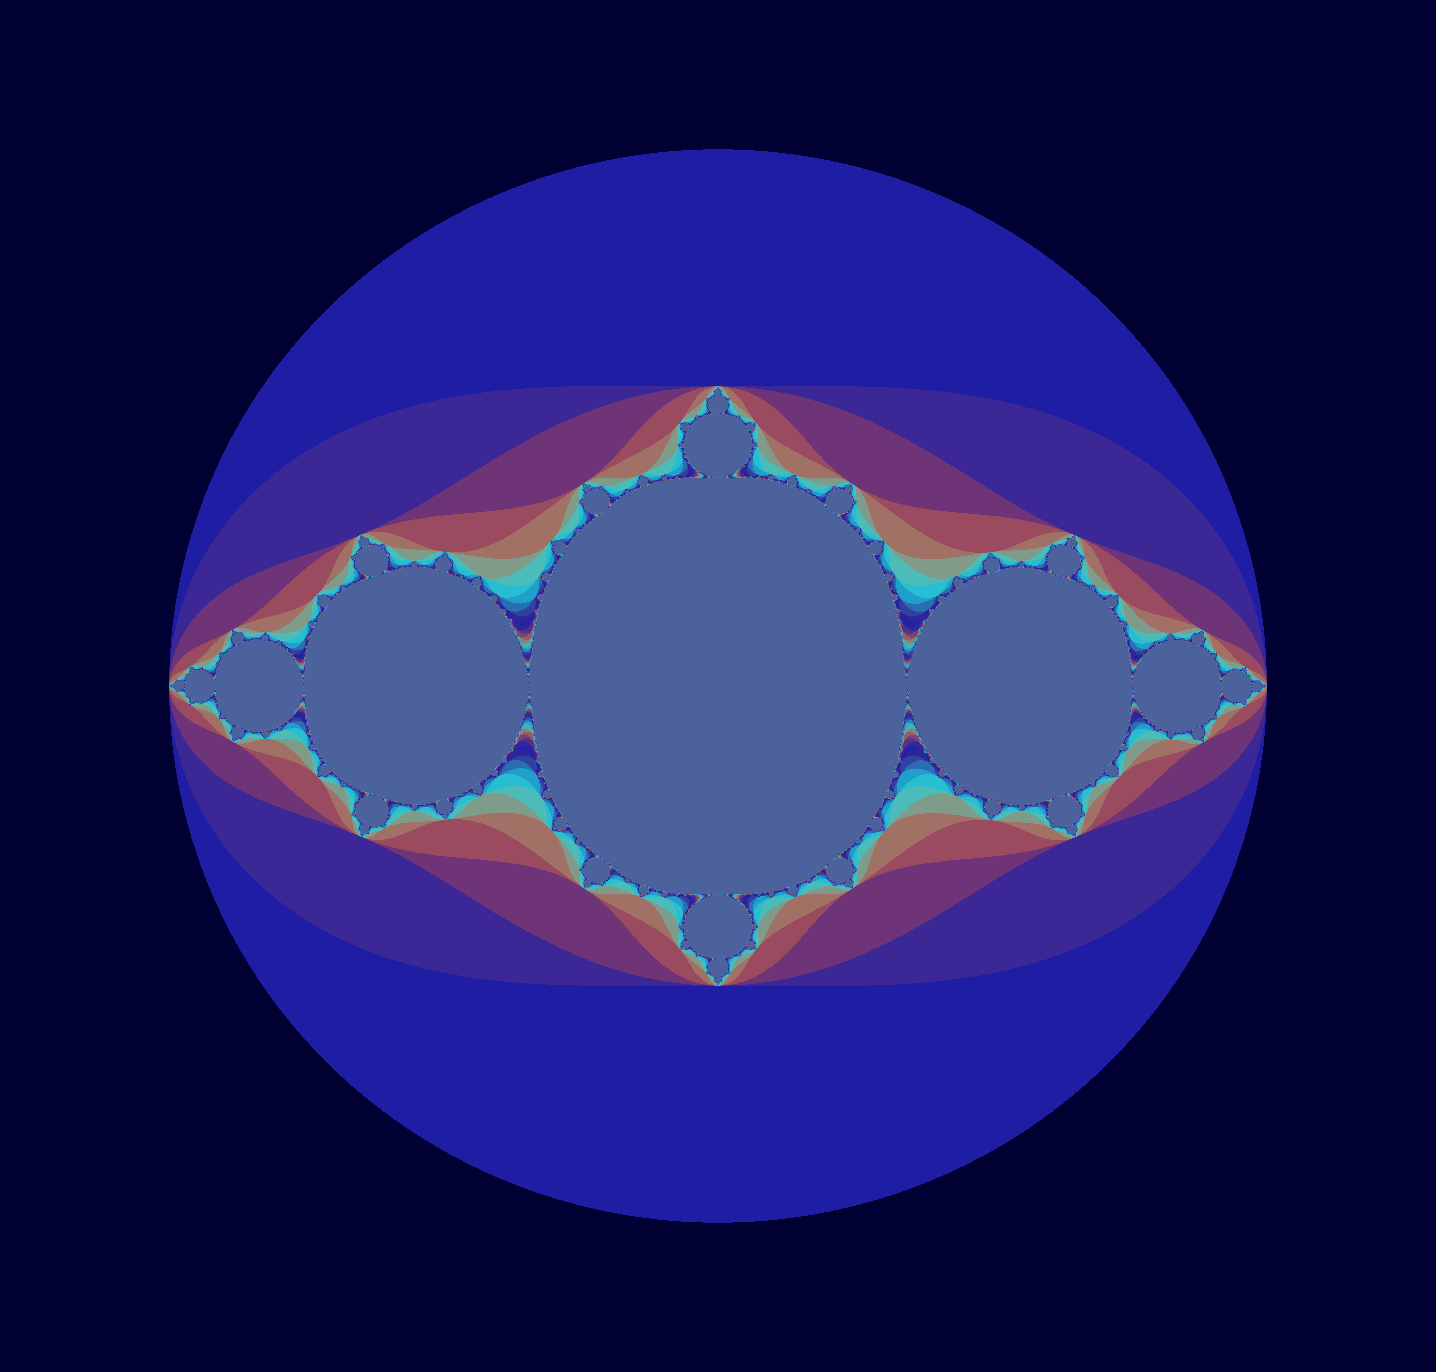
\includegraphics[width=\textwidth]{images/colorful3.png}
    \end{subfigure}
    \hfill
    \begin{subfigure}[b]{0.45\textwidth}
        \centering
        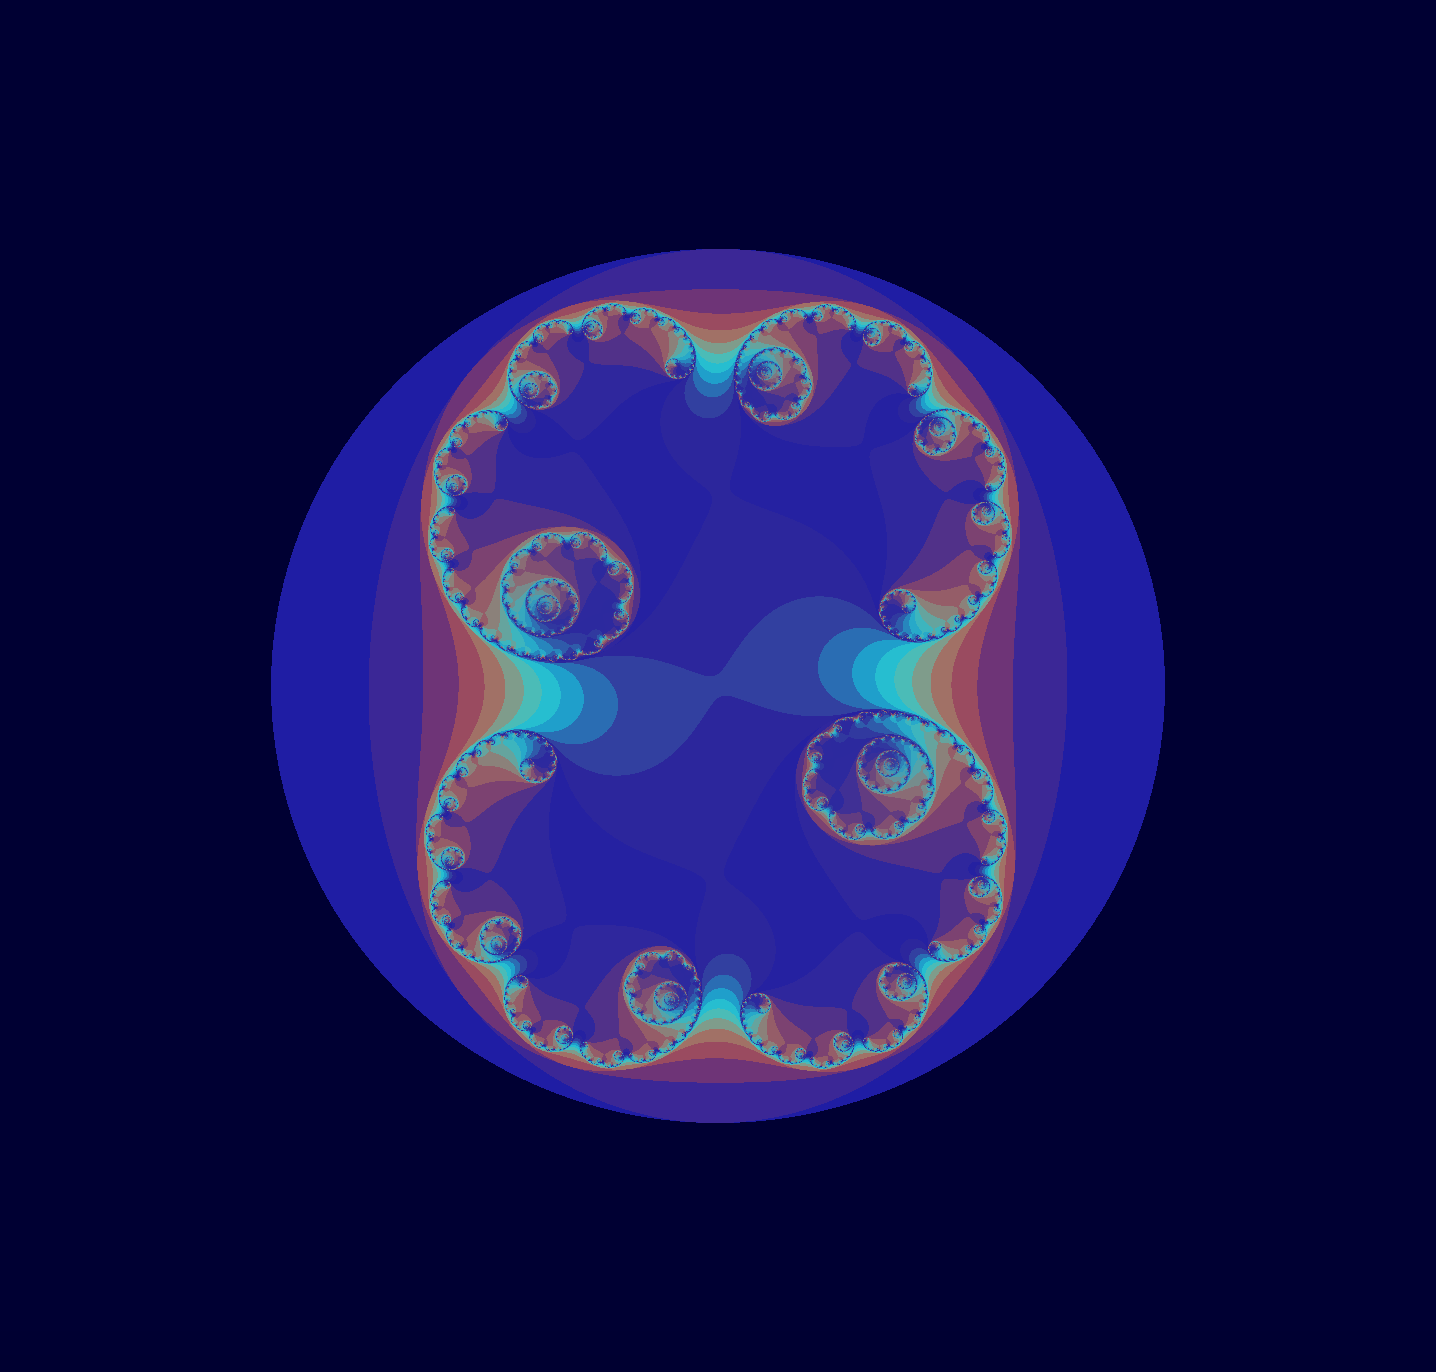
\includegraphics[width=\textwidth]{images/colorful4.png}
    \end{subfigure}
    \vskip\baselineskip
    \begin{subfigure}[b]{0.45\textwidth}
        \centering
        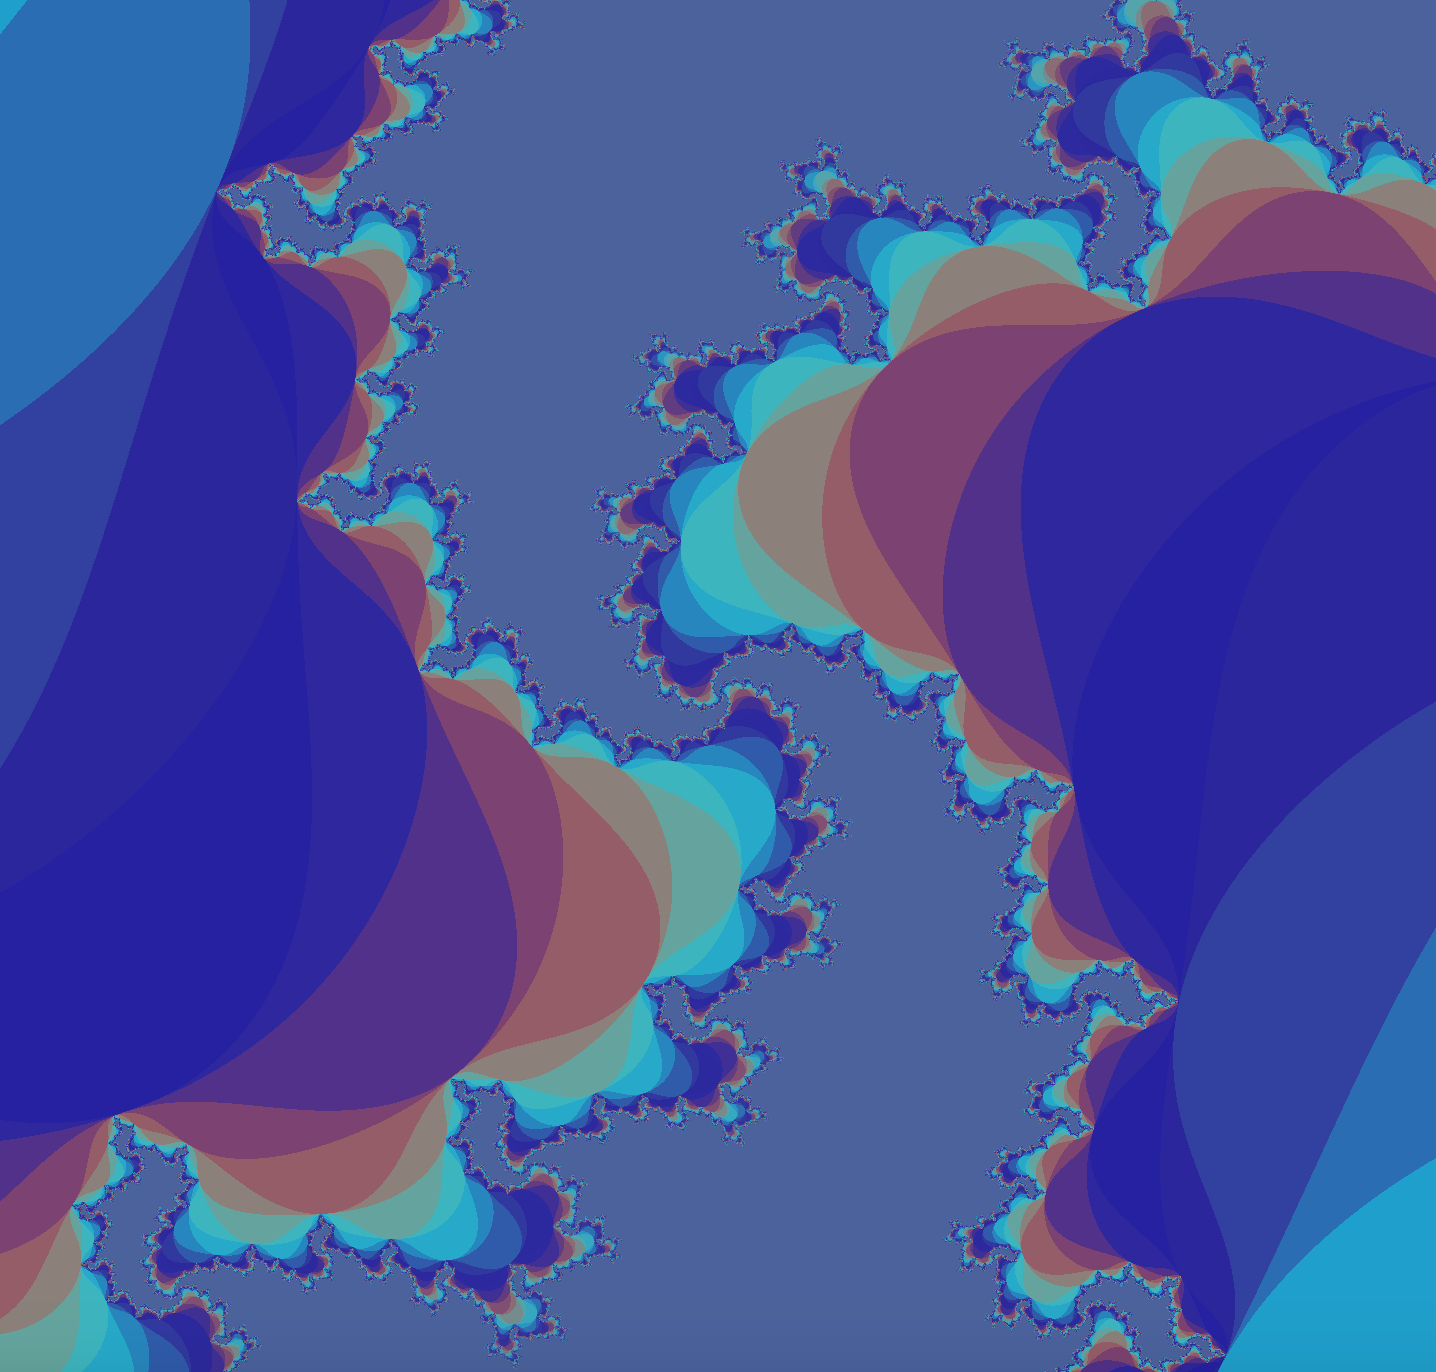
\includegraphics[width=\textwidth]{images/colorful5.png}
    \end{subfigure}
    \hfill
    \begin{subfigure}[b]{0.45\textwidth}
        \centering
        
\includegraphics[width=\textwidth]{images/colorful6.png}
    \end{subfigure}
    \caption{Neki primjeri iscrtanih Julijevih skupova u načinu rada 
        \emph{colorful}.}
    \label{fig:program_example}
\end{figure}

\section{Implementacijski detalji}

Program je implementiran koristeći tehnologiju \emph{OpenGL} koristeći 
programski jezik \emph{Julia}.
Da bi se iscrtala slika za svaki slikovni element određuje se $z_0$. Zatim se 
procjenjuje divergira li niz za određeni $z_0$ i na temelju toga se boja 
odgovarajući slikovni element. Za ovo je pogodno koristiti sjenčare budući da je
divergencija niza za pojedini slikovni element potpuno nezavisna od ostalih 
slikovnih elemenata, pa je posao lako paralelizirati. Zbog toga je iscrtavanje 
vrlo brzo, i animacija se bez poteškoća odvija u stvarnom vremenu.

Da bi se procijenilo divergira li niz za neki $z_0$, iterativno se određuju 
njegovi članovi. Ako za neki $z_n$ vrijedi $|z_n| > R$, gdje je
$$R = \frac{1 + \sqrt{1 + 4|c|}}{2},$$
tada znamo da niz divergira i nema smisla raditi daljnje iteracije. U nekom 
trenutku treba stati s iteracijama i tada niz proglašavamo ograničenim (iako on
to ne mora biti jer je moguće da tek za veliki $n$ vrijedi $|z_n| > R$). Boja 
slikovnog elementa određuje se na temelju broja iteracija potrebnih da se pokaže
divergencija. Moguće su razne strategije dodjele boje, ali u glavnom se radi o
načelu pokušaja i pogrešaka, a krajnja strategija uvelike ovisi o ukusu autora.

Jedna od mogućih strategija je definiranje pravokutnika gdje se svakom vrhu 
dodjeljuje neka proizvoljna boja. Može se definirati funkcija $c: \mathbb{N} 
\rightarrow \mathbb{R}^2$ koja određenom broju iteracija pridružuje par realnih 
brojeva
$$(x, y) = c(i).$$
Na temelju dobivenih $x$ i $y$ i odabranih točaka pravokutnika bilinearnom 
interpolacijom određuje se konačna boja. Na slici \ref{fig:program_example} 
korištena je funkcija
$$c(i) = e^{-\gamma_c i}(\cos(\omega_c i), \sin(\omega_c i)),$$
gdje su $\gamma_c$ i $\omega_c$ neki parametri, a točke pravokutnika su 
$(1, 1)$, $(-1, 1)$, $(-1, -1)$ i $(1, -1)$.

\section{Upute za pokretanje}

Program je testiran na računalu s operativnim sustavom \emph{macOS} 10.15.7 i 
i programskim jezikom \emph{Julia} verzije 1.5.3. Za pokretanje su potrebni 
moduli jezika \emph{Julia} \emph{CSyntax}, \emph{GLFW} i \emph{ModernGL}.

Nakon pozicioniranja u direktorij s izvornim kodom \texttt{juliaset.jl}, program 
iz naredbenog retka s dva argumenta:

$$\texttt{julia juliaset.jl <r> <način rada>}$$

gdje je $\texttt{<r>} = |c|$, a način rada može biti \texttt{colorful} ili 
\texttt{bw}. U direktoriju se moraju nalaziti i datoteke 
\texttt{fragment\_shader\_bw.glsl}, \texttt{fragment\_shader\_colorful.glsl} i 
\texttt{vertex\_shader.glsl}.

\begin{thebibliography}{2}

\bibitem{juliaset} Julia set, \url{https://en.wikipedia.org/wiki/Julia\_set}

\bibitem{mandelbrotset} Mandelbrot set, 
\url{https://en.wikipedia.org/wiki/Mandelbrot\_set}

\end{thebibliography}

\end{document}